\chapter{Fase geométrica en JCM generalizado}
\label{ch5:fgdoble}

%CAMBIAR ESTO PARA PERSONALIZARLO A MI GUSTO
\pagestyle{fancy}
\fancyhf{}
\fancyhead[LE]{\nouppercase{\rightmark\hfill}}
\fancyhead[RO]{\nouppercase{\leftmark\hfill}}
\fancyfoot[LE,RO]{\hfill\thepage\hfill}

\section{FG unitaria}

\section{FG disipativa}
VER SI PUEDO PONER LAS ECUACIONES DIFERENCIALES DE LOS ELEMENTOS DE MATRIZ, Y PONER LA SOLUCION FORMAL DE AUTOVECTORES Y AUTOVALORES DE 3X3, PARA SACAR UNA EXPRESION FORMAL DE LA FG EN TERMINOS DE LOS ELEMENTOS DE matriz
Al igual que en la sección \ref{sec3:jcm disipativo}, se estudia la dependencia de la fase geométrica en los distintos parámetros del problema. Se estudian los efectos en cada caso, y se buscan condiciones de robustez. Nuevamente, se estudiaran las condiciones iniciales $\ket{eg0+ge0}$, $\ket{eg1+ge1}$ y $\ket{3ero}$, con el objetivo de recuperar comportamientos similares al JCM de 1 átomo para el primer caso, y comparar estos con la segunda condición inicial. \textcolor{red}{$\ket{3ero}$ ???}.
\subsection{Dependencia con el régimen de acoplamiento}
En la figura \ref{fig5:dependencia acoplamiento} se observa la fase geométrica acumulada para diferentes valores del acoplamiento con el entorno $\gamma=0, 0.01g,0.1g,0.5g,g$, donde cada valor se corresponde con una curva mostrada, en orden ascendente en los colores, es decir, $\gamma=0$ se corresponde con el azul oscuro, y $\gamma=g$ se corresponde con el color mas claro, el naranja. Vemos como el comportamiento para el primer caso (\ref{fig5:dependencia acoplamiento eg0}) es idéntico al caso del JCM de 1 átomo, donde aumentar la disipación hace que los escalones se suavicen, y dejen de acumular fase mas rápidamente. 

\begin{figure}[h]
    \centering
    \begin{subfigure}{0.49\textwidth}
        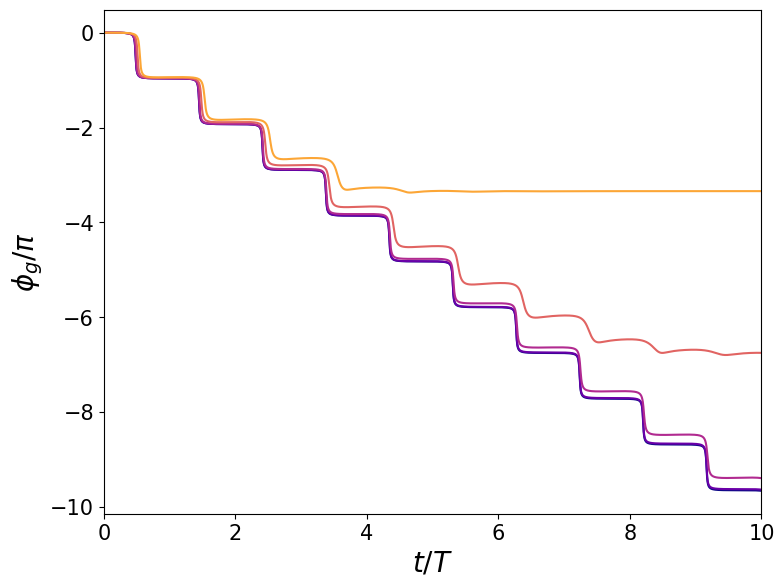
\includegraphics[width=\textwidth]{figuras/ch5/dependencia/eg0+/acoplamiento d=0.1g.png}
        \caption{$\ket{eg0+ge0}$}
        \label{fig5:dependencia acoplamiento eg0}
    \end{subfigure}
    \hfill
    \begin{subfigure}{0.49\textwidth}
        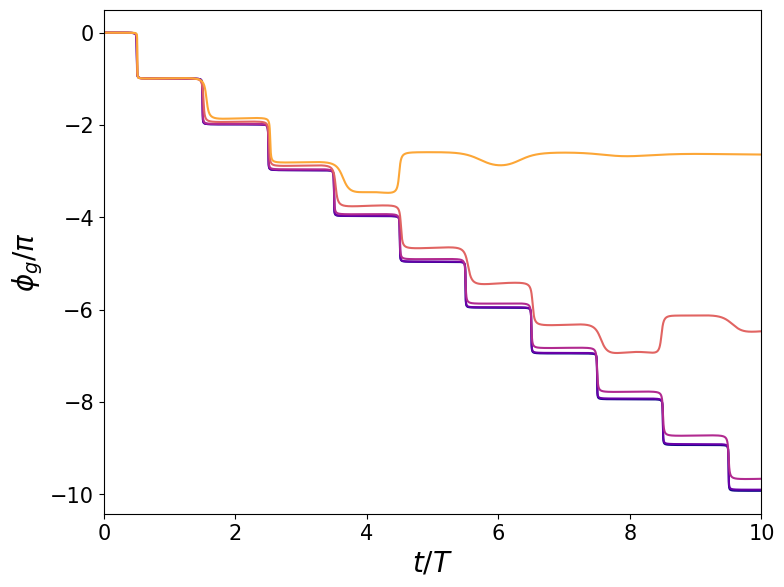
\includegraphics[width=\textwidth]{figuras/ch5/dependencia/eg1+/acoplamiento d=0.1g.png}
        \caption{$\ket{eg1+ge1}$}
        \label{fig5:dependencia acoplamiento eg1}
    \end{subfigure}
    \caption{Dependencia con el acoplamiento con el entorno}
    \label{fig5:dependencia acoplamiento}
\end{figure}
En el caso de la condición inicial correspondiente a el subespacio de $N=2$, se observa un nuevo comportamiento, y es un \textit{rebote}. Al aumentar lo suficiente el acoplamiento con el entorno, la acumulación de fase geométrica hace un salto en la dirección contraria a la que lleva normalmente, y luego se queda en un mismo valor. Recordemos que como se vio anteriormente, los saltos que hacen aparecer los escalones, se podían interpretar en el caso de 1 átomo utilizando la esfera de Bloch; estos saltos ocurren cuando la trayectoria llega al otro lado de la esfera de Bloch, y al llegar al lado opuesto (digamos $\phi=\pi$), justo al superar este punto, el camino mas corto para cerrar el ciclo según la regla de la geodésica es recorrer la esfera por el otro lado, dando así un salto de $\pi$ en el caso resonante. Esta interpretación en el caso de un espacio de Hilbert mas extenso no es tan directa, pero se puede pensar en analogía en una esfera de mayor dimensión, en donde entonces, el rebote seria una situacion similar a la descrita anteriormente, pero en otro hiperplano de la hiperesfera donde ocurre la trayectoria del estado. Mas allá de esto, el comportamiento es el esperado, e incluso vemos que ambos casos acumulan una fase geométrica muy similar en términos de su valor absoluto. No parece haber diferencias significativas en la influencia que tiene el entorno sobre estos dos estados.
\subsection{Dependencia con el detunning}
delta list=(0.00001*g,0.1*g,0.500001*g,1.00001*g,1.500001*g,2.5*g,5*g)

Para estudiar el efecto del detunning sobre la fase geométrica, se dejan fijos los otros parámetros del problema y se varia la diferencia entre las frecuencias de los átomos y la cavidad. Como el régimen de acoplamiento fuerte es el que nos interesa, se elije un acoplamiento con el entorno $\gamma=0.1g$ y $p=0.005g$, y en un principio los demás parámetros en cero $\chi=k-J=0$. En la figura \ref{fig5:dependencia detunning} se muestran la fase acumulada para diferentes valores del detunning $\Delta$ para las dos condiciones iniciales elegidas. En \ref{fig5:dependencia detunning eg0} se observa el mismo comportamiento que en el caso de 1 átomo, el detunning hace que las escalones sean mas suaves y el salto menor, haciendo que en conjunto el sistema acumule poca fase geométrica. Si asociamos la fase geométrica al camino que recorre el estado en el espacio de parámetros, es evidente que a mayor detunning, la fase acumulada sera menor, ya que como se menciono en reiteradas ocasiones, al aumentar el detunning las oscilaciones entre los estados son muy pequeñas, y por lo tanto la probabilidad esta concentrada en la condición inicial. Consecuentemente, en el espacio de parámetros, la curva se mantiene cerca del origen y por lo tanto la fase acumulada es menor. En el caso de la condición inicial en el subespacio de $N=2$, vemos que si el detunning es muy bajo, entonces el efecto es similar al anterior y la fase acumulada tiene una forma similar y también un valor similar. Pero cuando aproximadamente en el rango de  $1g \leq \Delta \leq 5g$, vemos que hay una gran diferencia. La fase acumulada es mas errática y presenta saltos y \textit{rebotes}, y pero al ir aumentando el detunning, estos parecen disminuir y converger al comportamiento esperado para un detunning muy grande: que la fase acumulada sea poca.
\begin{figure}[h]
    \centering
    \begin{subfigure}{0.49\textwidth}
        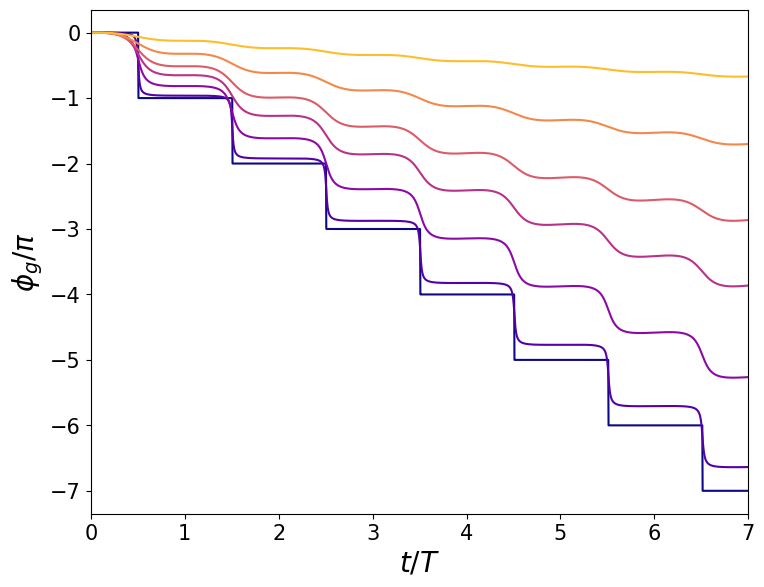
\includegraphics[width=\textwidth]{figuras/ch5/dependencia/eg0+/detunning todo 0.png}
        \caption{$\ket{eg0+ge0}$}
        \label{fig5:dependencia detunning eg0}
    \end{subfigure}
    \hfill
    \begin{subfigure}{0.49\textwidth}
        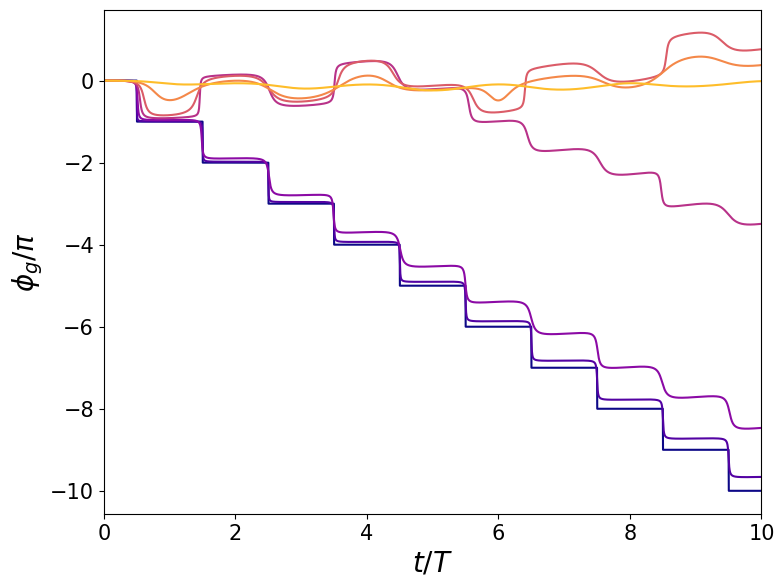
\includegraphics[width=\textwidth]{figuras/ch5/dependencia/eg1+/detunning todo 0.png}
        \caption{$\ket{eg1+ge1}$}
        \label{fig5:dependencia detunning eg1}
    \end{subfigure}
    \caption{Dependencia con el detunning}
    \label{fig5:dependencia detunning}
\end{figure}
Esto se debe a que entre estos valores del detunning, las poblaciones comienzan a presentar batidos. Las probabilidades de los estados $\ket{ee0}$ y $\ket{gg2}$ comienzan a aumentar y son comparables a la probabilidad del estado inicial. Esto hace que en el espacio de estados, las curvas sean complicadas y tengan trayectorias largas, haciendo que en algunos casos el salto sea positivo, y en otros negativo. Para valores de detunning bajos, el sistema principalmente se centra en el estado $\ket{eg1+ge1}$, y para detunnings altos también. Es en este rango intermedio, donde las amplitudes de los 3 estados sin similares y oscilan de manera errática, presentando batidos, y por eso es en este rango que la fase geométrica acumulada es impredecible. 
No se encontró una manera esquemática y clara de representar esto en el espacio de parámetros para poder entender intuitivamente el comportamiento, ya que la esfera de Bloch no es una herramienta que se pueda utilizar en esta situación. 
Para seguir el estudio, se presenta la diferencia entre la fase geométrica unitaria y la disipativa en función del detunning, para esto se realizan simulaciones para diferentes valores de $\Delta$ y se compara el valor de la fase geométrica luego de un tiempo fijo $t=3T$ para dos casos, el primero presentando perdidas y el segundo sin perdidas. Luego se realiza la resta de ambas cantidades y se obtiene el gráfico \ref{fig5:robustez detunning eg0}.

\begin{figure}[h]
    \centering
    \begin{subfigure}{0.49\textwidth}
        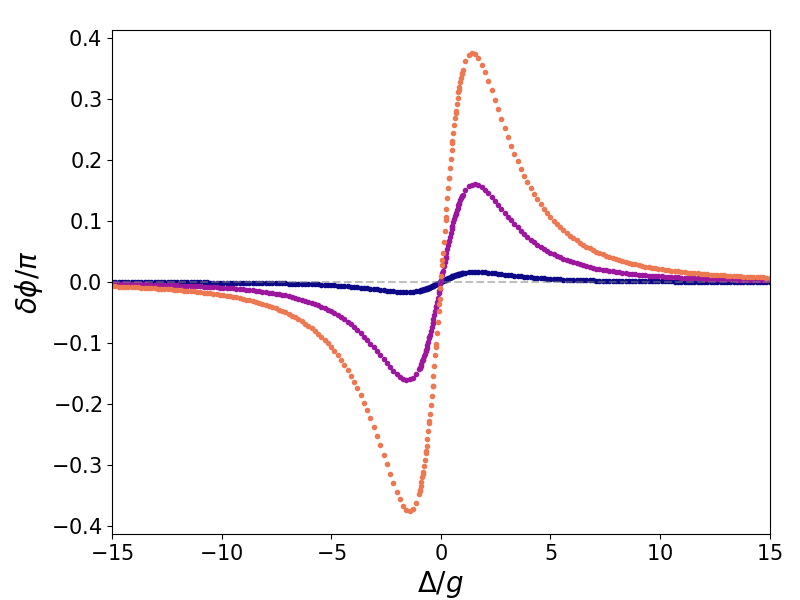
\includegraphics[width=\textwidth]{figuras/ch5/robustez/delta/eg0+ge0 k=0.0g x=0.0g J=0.0g.png}
        \caption{$\chi=0$}
        \label{fig5:robustez detunning 1 eg0}
    \end{subfigure}
    \hfill
    \begin{subfigure}{0.49\textwidth}
        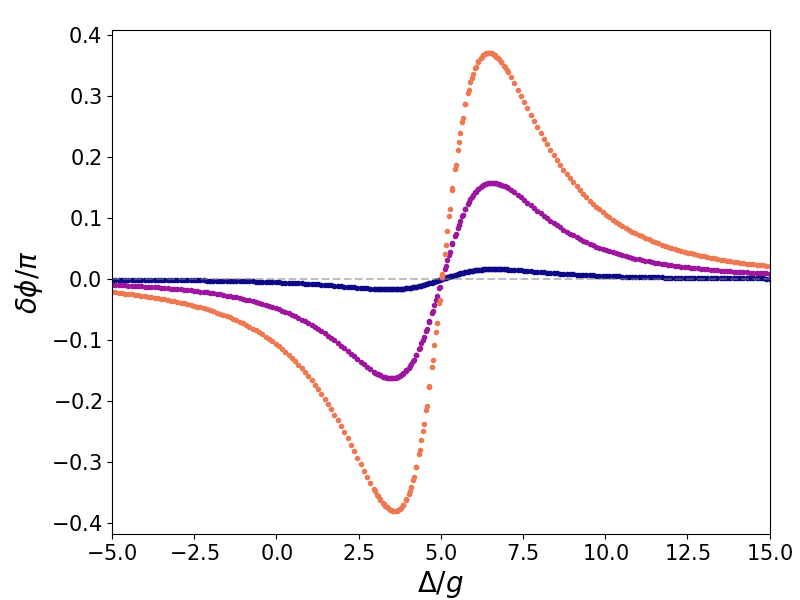
\includegraphics[width=\textwidth]{figuras/ch5/robustez/delta/eg0+ge0 k=0.0g x=5.0g J=0.0g.png}
        \caption{$\chi=5g$}
        \label{fig5:robustez detunning 2 eg0}
    \end{subfigure}
    \vfill

    \caption{Robustez en funcion de $\Delta$ para la condicion inicial $\ket{eg0+ge0}$}
    \label{fig5:robustez detunning eg0}
\end{figure}

En este se muestran 3 curvas diferentes correspondientes a 3 valores diferentes del acoplamiento con el entorno, respectivamente caracterizados por $\gamma=0.01g,0.1g$ y $0.25g$, y la condición inicial $\ket{eg0+ge0}$. En primer lugar, se ve que las 3 curvas pasan por el origen, lo que nos dice que la diferencia entre la fase geométrica en ambos casos es 0, que es lo que llamamos condición de robustez, ya que el entorno no tiene efecto sobre la fase geométrica y esta se mantiene robusta ante los efectos del entorno. En el panel \ref{fig5:robustez detunning 1 eg0}, correspondiente a $\chi=k-J=0$, la condición de robustez se da para $\Delta=0$, como era de esperarse ya que esta es la misma que para el caso de 1 átomo. De la misma manera, al observar el caso de $\chi=5g$ en la figura \ref{fig5:robustez detunning 2 eg0}, vemos que esta condición se da para $\Delta=\chi=5g$, que también es lo que esperamos. No hay mayores sorpresas. 

\begin{figure}[h]
    \centering
    \begin{subfigure}{0.49\textwidth}
        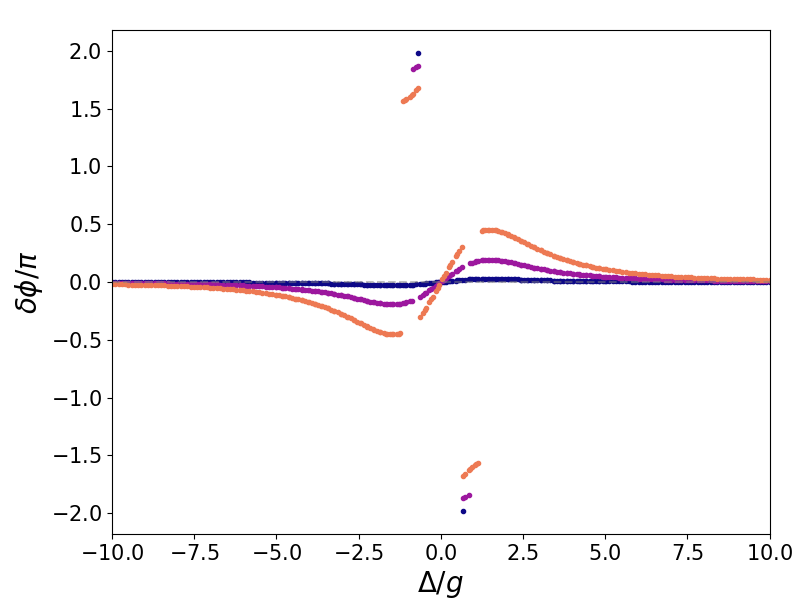
\includegraphics[width=\textwidth]{figuras/ch5/robustez/delta/eg1+ge1 k=0.0g x=0.0g J=0.0g.png}
        \caption{$\chi=0$}
        \label{fig5:robustez detunning 1 eg0}
    \end{subfigure}
    \hfill
    \begin{subfigure}{0.49\textwidth}
        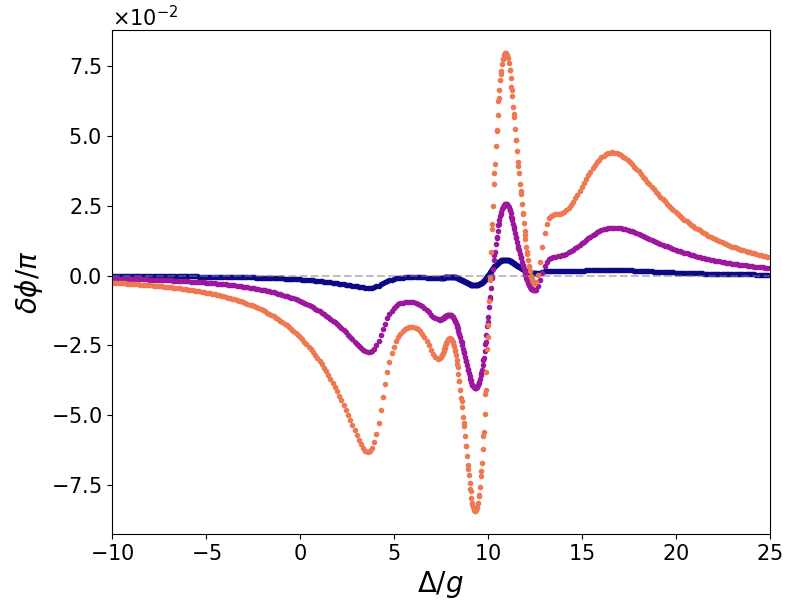
\includegraphics[width=\textwidth]{figuras/ch5/robustez/delta/eg1+ge1 k=0.0g x=5.0g J=0.0g.png}
        \caption{$\chi=5g$}
        \label{fig5:robustez detunning 2 eg0}
    \end{subfigure}
    \vfill

    \caption{Robustez en función de $\Delta$ para la condición inicial $\ket{eg0+ge0}$}
    \label{fig5:robustez detunning eg0}
\end{figure}

\subsection{Dependencia con el medio Kerr}
chi list=(0.0001*g,0.1*g,0.5*g,g,2*g,5*g)

La dependencia en el medio Kerr es interesante, ya que en el caso de 1 átomo se observo que el efecto del medio sobre la fase es análoga al detunning, y en el caso de dos átomos, se observa en la figura \ref{fig5:dependencia kerr eg0} la condición inicial $\ket{eg0+ge0}$ que esto sigue siendo cierto para el subespacio de $N=1$. Pero en el caso de la figura \ref{fig5:dependencia kerr eg1} se muestra que el efecto sobre la condición inicial $\ket{eg1+ge1}$, en comparación con \ref{fig5:dependencia detunning eg1}, muestra diferencias en el régimen intermedio que se había definido aproximadamente para valores entre $1g \leq \chi \leq 5g$. Si bien la forma no es igual, es notable que el rango que se definió como \textit{intermedio} es el mismo. Entonces, podemos decir que si bien para $N=2$ el medio Kerr no es simplemente un corrimiento en el detunning, el comportamiento es similar. 

\begin{figure}[h]
    \centering
    \begin{subfigure}{0.49\textwidth}
        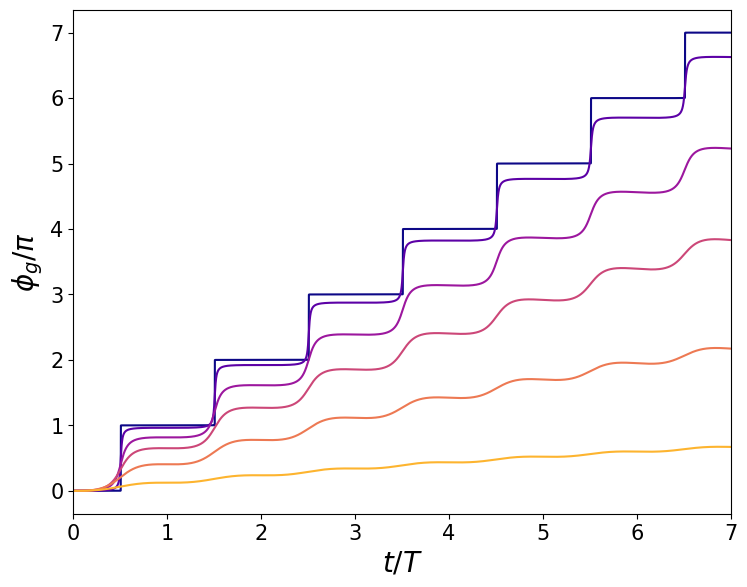
\includegraphics[width=\textwidth]{figuras/ch5/dependencia/eg0+/kerr todo 0.png}
        \caption{$\ket{eg0+ge0}$}
        \label{fig5:dependencia kerr eg0}
    \end{subfigure}
    \hfill
    \begin{subfigure}{0.49\textwidth}
        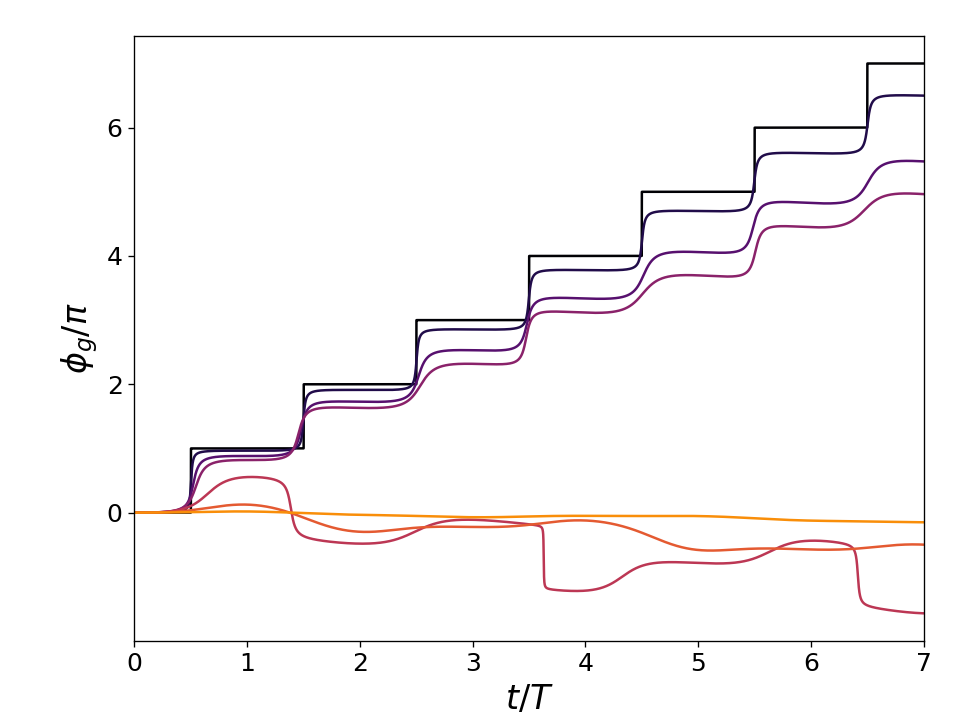
\includegraphics[width=\textwidth]{figuras/ch5/dependencia/eg1+/kerr todo 0.png}
        \caption{$\ket{eg1+ge1}$}
        \label{fig5:dependencia kerr eg1}
    \end{subfigure}
    \caption{Dependencia con el medio Kerr}
    \label{fig5:dependencia kerr}
\end{figure}

La pregunta que surge de todas formas es, que sucede si realizamos un corrimiento en el detunning. En el caso de 1 átomo se había observado como la condición de robustez se cumplía cuando $\Delta=\chi(2n-1)$, y la dependencia de la fase geométrica parecía no cambiar, solo presentaba un corrimiento. En este caso sera igual?
En la figura \ref{fig5:dependencia kerr 2 eg0} se observa como en el primer caso, aumentar el detunning hace que las primeras curvas, que representan valores de $\chi=0$ y $\chi=0.1g$ (en azul oscuro y violeta oscuro respectivamente), acumulan fase negativa y los saltos son suaves. Ahora, la curva de $\chi=\Delta=0.5g$ es igual a la de $\chi=\Delta=0$, y a partir de esta, el comportamiento es el mismo que antes. Pero para el caso de $N=2$, vemos como esto no es así. Primero, los casos de $\chi=0,0.5g$ ahora tienen saltos mas abruptos, y hay un rebote. Por otro lado, el caso robusto ya no se observa para $\chi=0.5g$, y en el rango intermedio, las oscilaciones de la fase parecen tener mas de una componente de frecuencia. Esto se observa claramente en la curva roja, donde se ve como hay dos saltos diferentes; uno es mas pronunciado seguido de otro mas pequeño. Esto nos indica que las condiciones \textcolor{red}{4.18/4.19} que se encontraron haciendo analogías con el caso de 1 átomo, no representan exactamente el caso de robustez.

\begin{figure}[h]
    \centering
    \begin{subfigure}{0.49\textwidth}
        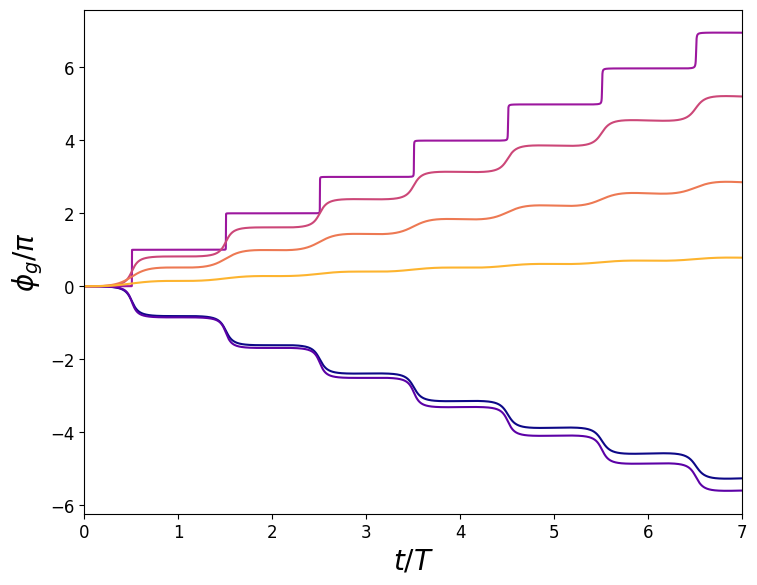
\includegraphics[width=\textwidth]{figuras/ch5/dependencia/eg0+/ker d=0.5g.png}
        \caption{$\ket{eg0+ge0}$}
        \label{fig5:dependencia kerr 2 eg0}
    \end{subfigure}
    \hfill
    \begin{subfigure}{0.49\textwidth}
        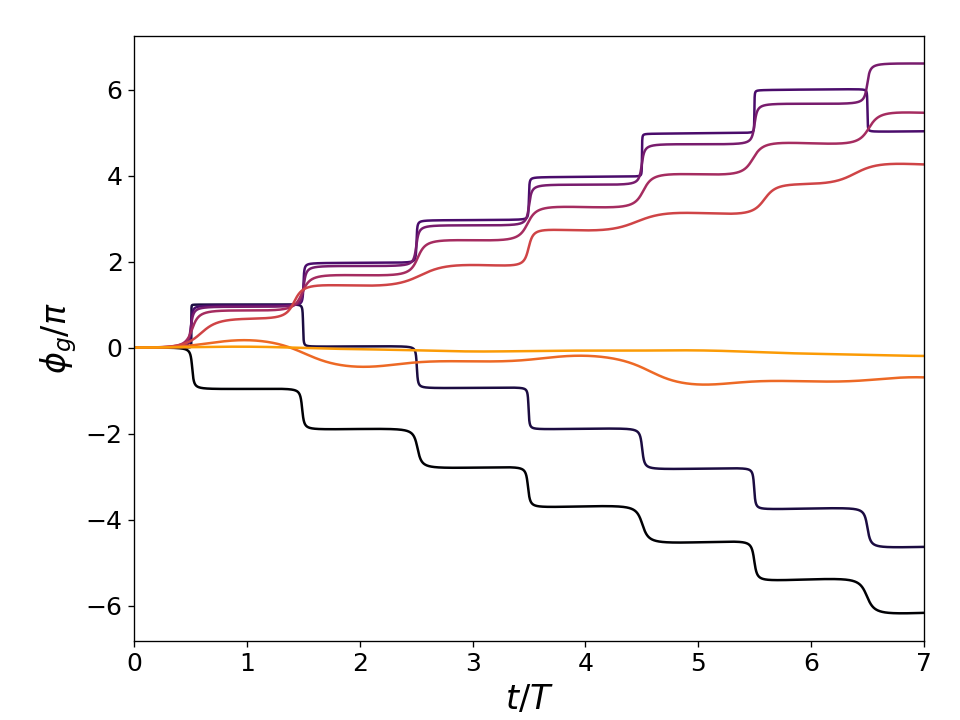
\includegraphics[width=\textwidth]{figuras/ch5/dependencia/eg1+/kerr d=0.5g.png}
        \caption{$\ket{eg1+ge1}$}
        \label{fig5:dependencia kerr 2 eg1}
    \end{subfigure}
    \caption{Dependencia con el medio Kerr con $\Delta=0.5g$}
    \label{fig5:dependencia kerr 2}
\end{figure}

Para confirmar esto, se realiza un gráfico de diferencias entre la FG unitaria y la disipativa en función del parámetro del medio. En la figura \ref{fig5:robustez kerr eg0} se muestra la diferencia $\delta\phi=\phi_d-\phi_u$ para la condición inicial $\ket{eg0+ge0}$. Se ve como la condición de robustez en este caso es igual que para el modelo de 1 átomo, donde la condición se da para $\Delta=\chi$. 

\begin{figure}[h]
    \centering
    \begin{subfigure}{0.49\textwidth}
        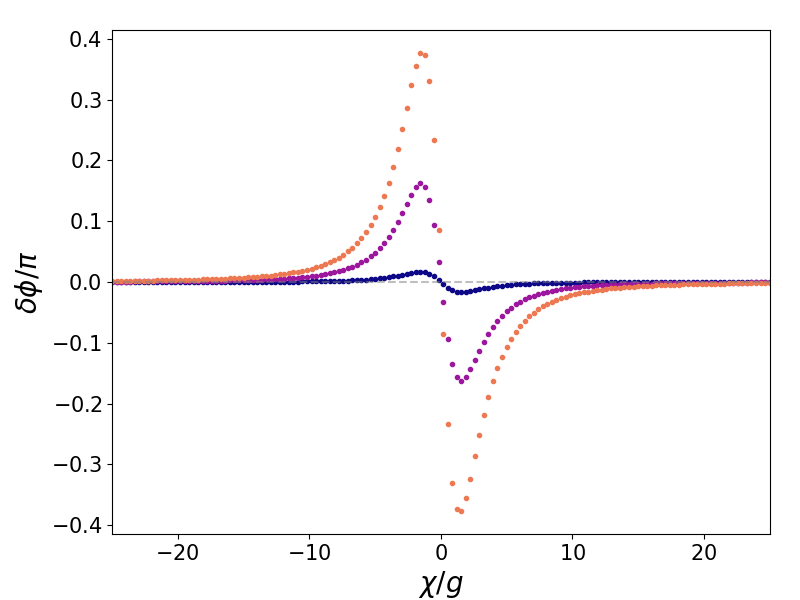
\includegraphics[width=\textwidth]{figuras/ch5/robustez/chi/eg0+ge0 d=0.0g k=0.0g J=0.0g.png}
        \caption{$\Delta=0$}
        \label{fig5:robustez kerr 1 eg0}
    \end{subfigure}
    \hfill
    \begin{subfigure}{0.49\textwidth}
        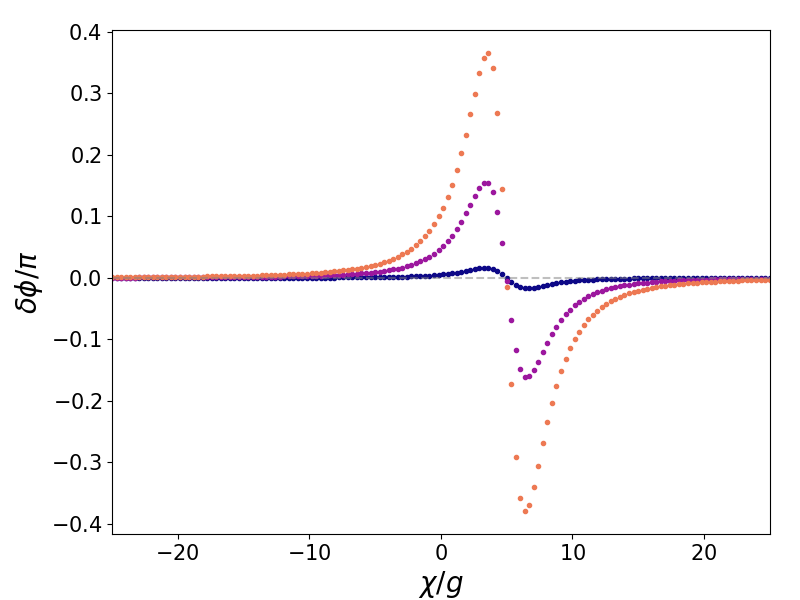
\includegraphics[width=\textwidth]{figuras/ch5/robustez/chi/eg0+ge0 d=5.0g k=0.0g J=0.0g.png}
        \caption{$\Delta=5g$}
        \label{fig5:robustez kerr 2 eg0}
    \end{subfigure}
    \caption{Robustez en función de $\chi$ para la condición inicial $\ket{eg0+ge0}$}
    \label{fig5:robustez kerr eg0}
\end{figure}

A diferencia del caso de $N=1$, si observamos la diferencia para el estado inicial $\ket{eg1+ge1}$ representada en la figura \ref{fig5:robustez kerr eg1}, entonces se ve como ahora no se cumple la analogía, y ademas hay mínimos y máximos locales que antes no había. 

\begin{figure}[h]
    \centering
    \begin{subfigure}{0.49\textwidth}
        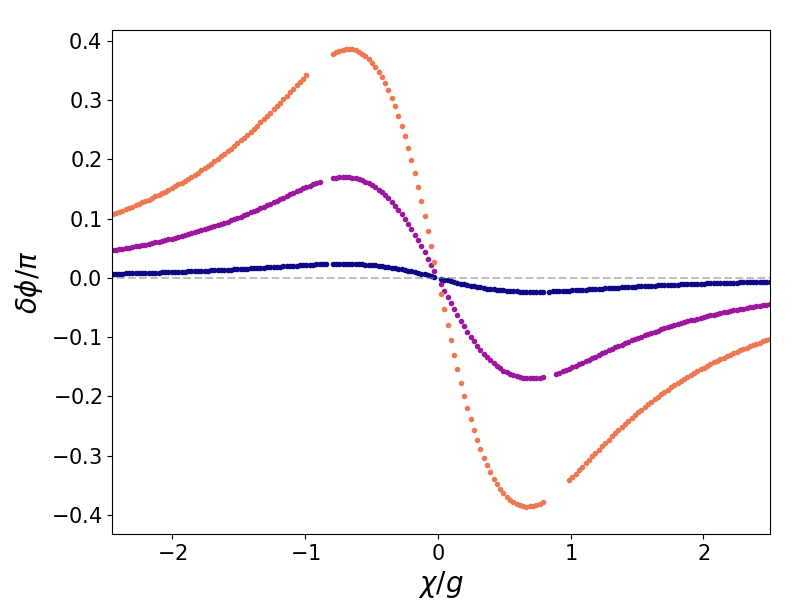
\includegraphics[width=\textwidth]{figuras/ch5/robustez/chi/eg1+ge1 chi zoom.png}
        \caption{$\Delta=0$}
        \label{fig5:robustez kerr 1 eg1}
    \end{subfigure}
    \hfill
    \begin{subfigure}{0.49\textwidth}
        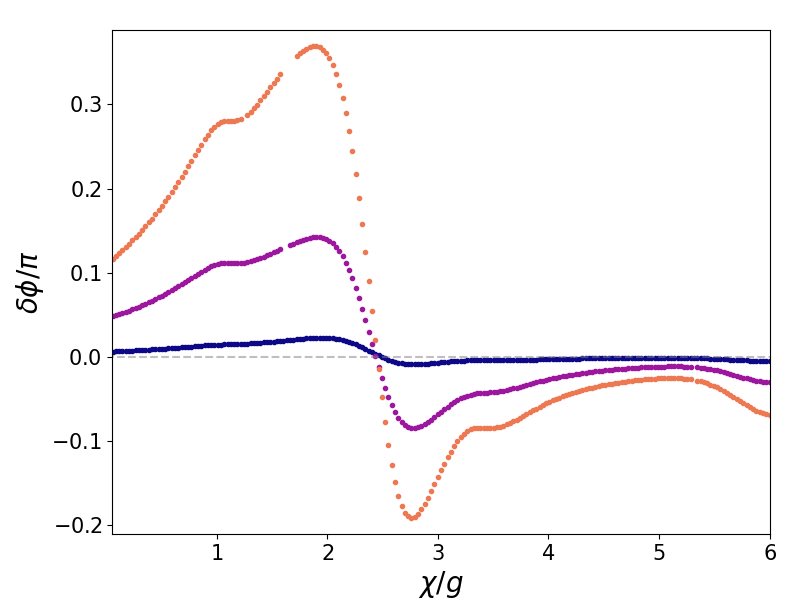
\includegraphics[width=\textwidth]{figuras/ch5/robustez/chi/eg1+ge1 chi d=5.0g.png}
        \caption{$\Delta=5g$}
        \label{fig5:robustez kerr 2 eg1}
    \end{subfigure}
    \caption{Robustez en función de $\chi$ para la condición inicial $\ket{eg1+ge1}$}
    \label{fig5:robustez kerr eg1}
\end{figure}


\textcolor{blue}{Lo primero que hay que aclarar, es que hay sitios en donde no hay puntos. En estos casos lo que sucede es que el medio, como es de comun conocimiento, introduce un corrimiento en las frecuencias, consecuentemente, hay un pequeño cambio entre la fase unitaria y la geometrica. En principio, esto no es un problema, ya que lo unico que hace es retrasar un poco el escalon. Pero en combinacion con la dinamica complicada del sistema, lo que ocurre en casos muy puntuales, es que la fase unitaria y la disipativa hacen un escalon en direcciones contrarias y esto hace que la diferencia entre ambas haga un salto discontinuo (o muy abrupto). En la figura \ref{fig5:robustez kerr 1 eg1} cerca de los valores $\chi/g=\pm 1$ se observan la falta de puntos, estos estan mas arriba por el salto que se menciono. Es tambien interesante, que no es solo para un caso aislado, sino que es en un rango de valores donde se observa este comporamiento, que luego se normaliza. }

Lo primero que se observa en la figura \ref{fig5:robustez kerr eg1} es que hay algunos lugares donde faltan puntos. Esto se debe a que el entorno tiene un efecto interesante para algunas combinaciones de parámetros, y es que en algunos casos en particular por ejemplo la fase geométrica unitaria presenta escalones ascendentes, y en general el caso disipativo es similar, pero en algunos casos, el entorno hace que el salto sea en la dirección contraria, lo que hace que la diferencia entere las fases tenga un salto abrupto. Entonces, los puntos que faltan en esta imagen, simplemente son regiones donde la diferencia es muy grande y no están representadas en este gráfico. En este caso, este comportamiento se da en la figura \ref{fig5:robustez kerr 2 eg1} para $\chi / g \sim \pm 1$. Este comportamiento se da no solo para un valor particular de los parámetros, sino para un rango, y este depende del acoplamiento con el entorno, ya que se observa que para la curva naranja perteneciente a $\gamma=0.25g$ el rango sin puntos es mayor a los otros dos. Esto fortalece la hipótesis que el entorno es responsable por este comportamiento.

En la figura \ref{fig5:robustez kerr 2 eg1} se muestra el caso en donde se aumento el detunning hasta $\Delta=5g$. Se observan máximos y mínimos locales en valores que no se pudieron predecir. Las dos cosas interesantes que se observaron son que también se encontraron regiones en donde se encuentran saltos en la diferencia por la misma razón que en el caso anterior, y por otro lado, y mas interesante aun, es que ahora la condición de robustez parece estar cercana a $\chi=2.5g$; si se acerca y se observa con detalle, se encuentra que en realidad el cero se encuentra en $\chi\sim 2.45g$ y varia suavemente con cada valor de $\gamma$. Esto es muy interesante, ya que el efecto que tiene el entorno también se refleja en esta condición.

\subsection{Dependencia con la interacción entre átomos}
k list=(0,0.1*g,0.5*g,g,2.5*g,5*g)


\begin{figure}[h]
    \centering
    \begin{subfigure}{0.49\textwidth}
        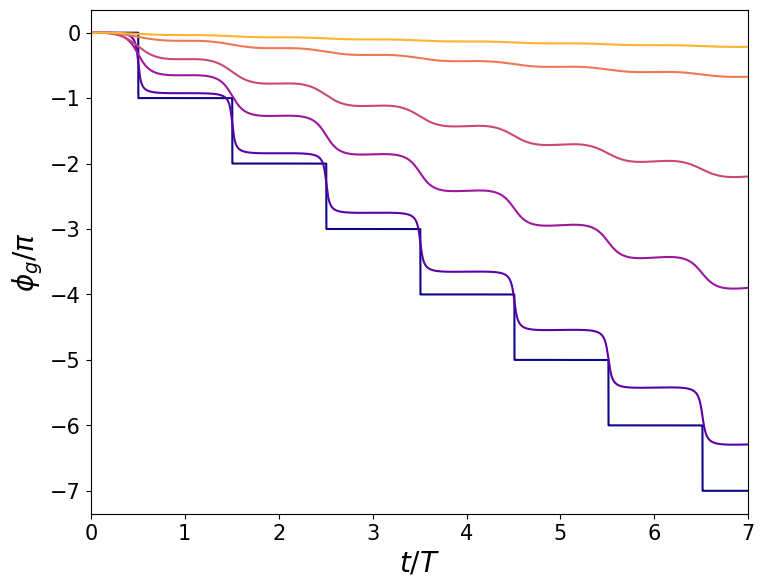
\includegraphics[width=\textwidth]{figuras/ch5/dependencia/eg0+/interaccion todo 0.png}
        \caption{$\ket{eg0+ge0}$}
        \label{fig5:dependencia interaccion eg0}
    \end{subfigure}
    \hfill
    \begin{subfigure}{0.49\textwidth}
        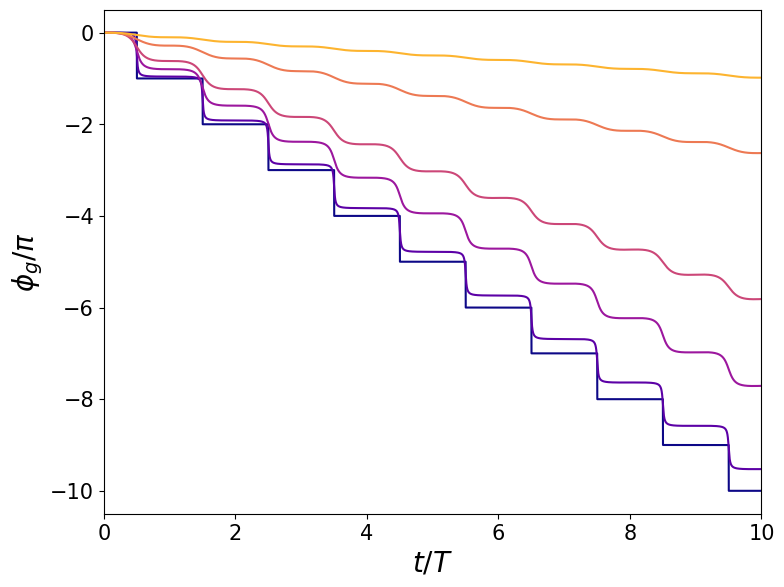
\includegraphics[width=\textwidth]{figuras/ch5/dependencia/eg1+/interaccion todo 0.png}
        \caption{$\ket{eg1+ge1}$}
        \label{fig5:dependencia interaccion eg1}
    \end{subfigure}
    \caption{Dependencia con la interacción entre los átomos}
    \label{fig5:dependencia interaccion}
\end{figure}
\subsection{Robustez}
Finalmente, por completitud, se explorara mas en detalle las condiciones de robustez en función del detunning. Esto es importante ya que este es en general el parámetro de control al que se tiene acceso en los experimentos, en general, cambiando la frecuencia de la cavidad.


